\section{Related work}
\begin{figure*}[htbp]
	\centering
	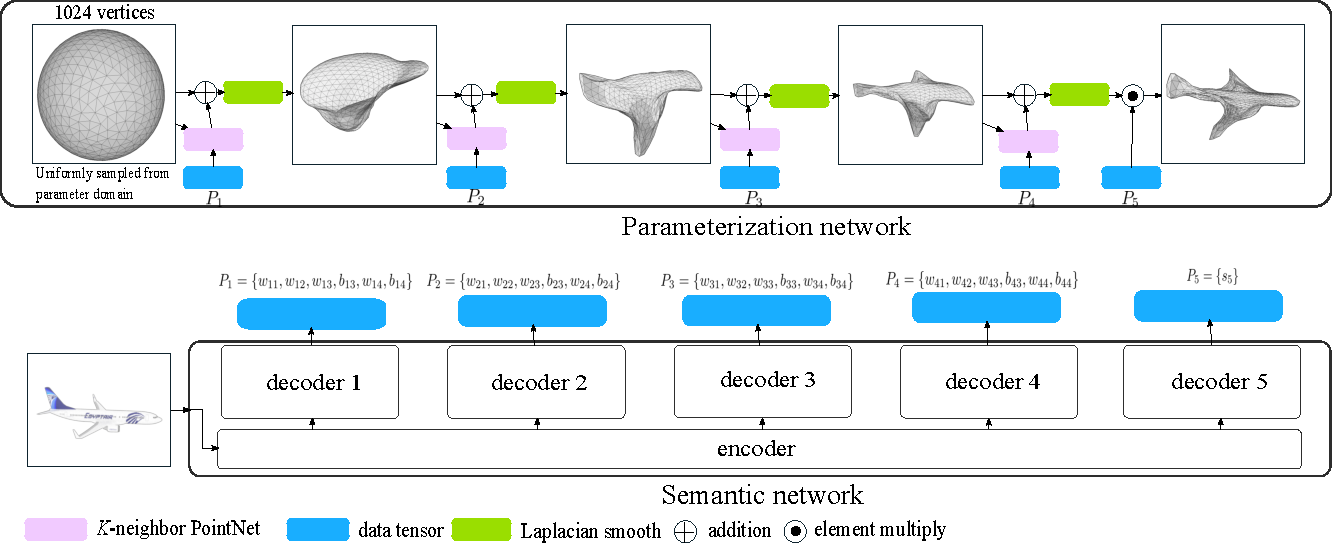
\includegraphics[width=\linewidth]{img/net/overview}
	\caption{The overview of the network: The proposed framework consists of two networks. One is the parameterization network that maps points sampled from parameter domain to target shape. The other is the semantic network that takes image as input and predict parameters for the parameterization network.}
	\label{fig:overview}
\end{figure*}
\subsection{Image based modeling}
\subsection{Deep shape generation}
3D shape is not canonical function which leads to multiple exploration in its representation for deep learning.

\noindent\textbf{Volume Occupancy}

\noindent\textbf{Point Cloud}

\noindent\textbf{Mesh}
\subsection{Parameterization in deep learning}
 The idea that utilize parameterization in the representation of 3D shape have been explored by the works of \cite{surfnet}\cite{geoimg}. As detailed as their output can be, the proposed methods involves a non-trainable procedure for the creation of geometry image. These methods also require manifold surface as training data so that the shapes can be parameterized using spherical parameterization and turned into geometry image. However, the public datasets like ShapeNet\cite{shapenetdata} contains meshes that are not manifold surfaces. Our method is trying to train a network that can predict the parameterization. We use point set which can easily be sampled from the non-manifold meshes as ground truth. 
\begin{comment}
\subsection{Learning to learn and filter prediction}
It is not a new idea to learn neural networks that predict the parameters of another. It is one of the approaches found for \textit{learning to learn}.  A few authors \cite{schmidhuber1992learning,bertinetto2016learning,jia2016dynamic} , in particular, have proposed to apply such idea in their works. Our work explore this idea under total different motivations. Our motivations are a) to relate the input image to proposed parameterization network b) to handle the \textit{sampling variation} and \textit{semantic variation} separately. 

\subsection{Networks for shape generation from image}
Recently, the network structure for shape generation from image is being actively exploring. One approach is to represent the shape as volumetric occupancy function. \cite{3DR2N2} proposed 3D-R2N2, a 3D recurrent neural network based on LSTM to infer a 3D volumetric function from a single view or multiple views. \cite{girdhar2016learning} proposed a network for single view shape generation by embedding the image and shape all together. \cite{NIPS2016_6096} applys the idea of VAE-GAN on the task of volumetric shape generation. \cite{NIPS2016_6206} uses only images contour as supervision for the shape generation and \cite{NIPS2016_6600} proposed a conditional generative network for unsupervised learning of shape generation. 

These neural networks use voxel representations, which
requires a large amount of memory and is inefficient respecting to common 3D transformations (i.e. rotation, affine transformation ). \cite{PSGN} proposed an alternative approach with neural networks that regress unordered
3D point sets for 3D shape generation. 

Our network also use point set as ground truth but we actually represent the shape as a spatial distribution in the form of a spherical uniform distribution plus a predicted mapping, which is total different from all the above methods. 

\subsection{Networks for shape deformation}
An alternative way for shape generation is to deform from given template to target shape. \cite{deformflow} use precomputed deformation offsets as ground truth to train a 3D convolutional neural network that generates a deformation field as an output for 3D mesh editing. \cite{Huang:2015:SRV:2809654.2766890} generate shape according to image through template retrieval and
deformation, which relies on jointly segmenting the 2D image and 3D templates and creating the 
3D generation from deformed parts of the segmented templates. A recent work on arXiv, \cite{deformnet}, propose a method of retrieval plus deformation network for the shape generation task. It introduce a differentiable deformation layer and it takes features from both the input image and the input template.
A even more recent work on arXiv, \cite{img2mesh}, propose a method that retrieve, deform and finally blend the mesh in dataset to target mesh. 
Our method relates to the above methods in the way that our parameterization network deforms the samples from the surface of unit sphere to the target surface. Its framework can only handle images from a specific category, while our network takes images from multiple categories.  
The above methods looking to start the deformation from good point set/mesh by retrieval. In such setting, the point set/mesh for retrieval serves as an external memory for the whole model. 
Our method differs from these method in the way that our network start the learning from scratch. Our template, the unit sphere, contains no prior knowledge for any target shape. It only serves as a parameter domain for sampling.
\end{comment}
